%%%%%
%%%%% Template for beamer presentation using FMI 2019 style
%%%%%
\documentclass[
    presentation,aspectratio=1610,
    hyperref={colorlinks,citecolor=blue,linkcolor=black,urlcolor=blue},
]{beamer}
% \documentclass[presentation]{beamer}

%% Use beamer FMI theme
\useinnertheme{rounded}
\usetheme{FMI}

% \subtitle{my subtitle}  % add subtitle
%\institute[IL]{Ilmatieteen laitos} % change institute

%\setbeamertemplate{footline}[numberonly] % only page number in footer
%\setbeamertemplate{footline}[empty] % only page number in footer

%% Select language
%\RequirePackage[finnish]{babel}
\RequirePackage[english]{babel}

%% Input coding, Latin1:
%\RequirePackage[latin1]{inputenc}
%\RequirePackage[T1]{fontenc}
% or UTF-8:
\RequirePackage[utf8]{inputenc}
\RequirePackage{fontenc}

\RequirePackage{graphicx}
\graphicspath{{./fig/}} % graphics searched from fig directory
\RequirePackage{amsmath}
\RequirePackage{bm}

\RequirePackage{appendixnumberbeamer}

\usefonttheme{professionalfonts}

%% Fonts, Helvetica, with Euler math
\RequirePackage{eulervm}  % Euler math
\RequirePackage[scaled]{helvet}

%% Multimedia support
\RequirePackage{multimedia}
% \RequirePackage{media9}

\setbeamercolor{block title}{bg=fmiblue,fg=white}
\setbeamercolor{block body}{bg=fmiblue!10,fg=black}

%% Title and Author
\title[]{Adjoint-based data assimilation of sea surface height for the Baltic Sea}
\author[T. Kärnä]{Tuomas Kärnä\inst{1}, Joe Wallwork\inst{2}, Stephan Kramer\inst{2}}
\institute[]{\inst{1} Finnish Meteorological Institute \\ \inst{2} Imperial College London}
\date{\vspace*{6mm} Ocean Sciences Meeting, March 2, 2022}

\definecolor{crimson}{HTML}{DC143C}

\begin{document}

%% Main title page, automatically generated, use outside frame or make your own title page
\maketitle

% - mesh: 53k triangles, 260k elevation points
% - wrt Nemo-Nordic 310k elevation points
% - shallow water equations
% - fully implicit solver, 2nd order two-stage Runge-Kutta (DIRK22)
% - 1 h time step
%
% - EMODNET 2020 bathymetry
% - Harmonie atmospheric forcing, msl pressure, 10 winds
% - River discarge, climatology, (E-HYPE forecast coming)
% - TPXO 9 tidal model at boundary
%
% - CSC Mahti 8 CPUs
% - 1800x realtime: 3 months takes 45 min
% - optimization period: June 1 .. June 17, 2019
% - validation period: June .. August 31, 2019
% - one optimization iteration takes ~4x
% - 17 d forward run: 12 min, iteration 48 min


% simulation: outputs_m014_28-i40
% - 63 stations
% -

% 15 mins recorded presentation
%
% ~ 10 slides
%
% Outline slide
%
% Adjoint-based data assimilation: pros and cons
% -
%
% Automated generation of adjoint model
% -
%
% Firedrake-adjoint
% -
%
% Application to Baltic Sea water elevation modeling
% - Different tidal/non-tidal regimes
%
% Model domain and configuration
% - bathymetry, mesh, forcings
%
% Animation SSH
% - Tides are filtered out in the Danish Straits
%
% Tide gauges, cost function, control
% -
%
% Regularization
% -
%
% Optimization results
% - metrics
% - Optimized Manning field
% Examples of time series
%
% Discussion
% - model must be accurate; error dominated by the control variable
% - cost function must be carefully chosen
% - best way to regularize is to increase opt period run time
% - additional regularization for control
%
% Future work
% -

\frame{
\frametitle{Adjoint-based inverse modeling}
% \vspace*{-6mm}
\begin{columns}
 \column{0.48\textwidth}
 Why inverse modeling?
 \begin{itemize}
  \item Amount of observational data is increasing
  \item Need for automated methods to combine observations and models
  \item Parameter estimation, model state estimation, sensitivity analysis, error quantification, ...
 \end{itemize}
 \textbf{Parameter estimation}
 \begin{itemize}
  \item Manual model calibration can be very time consuming
 \end{itemize}
 \column{0.53\textwidth}
 Adjoint model
 \begin{itemize}
  \item Compute the sensitivity of model output versus \emph{any} model parameter
  \item[+] Accurate
  \item[+] No need to run model ensembles
  \item[+] Cost does not depend on the number of model parameter
  \item[-] Adjoint model is tedious to implement
  \item[-] Needs to run backwards in time
 \end{itemize}
\end{columns}
}

% \frame{
% \frametitle{Adjoint-based data assimilation: pros and cons}
% % \vspace*{-6mm}
% \begin{columns}
%  \column{0.48\textwidth}
%  Pros
%  \begin{itemize}
%   \item
%  \end{itemize}
%  Cons
%  \begin{itemize}
%   \item Adjoint model is difficult to implement
%  \end{itemize}
%  \column{0.53\textwidth}
%   % \includegraphics[width=\textwidth]{domain_full}
% \end{columns}
% }

{\bgempty
\frame{
\frametitle{Automated generation of an adjoint model}
\begin{center}
 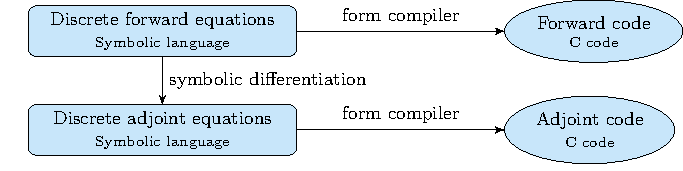
\includegraphics[width=0.7\textwidth]{figure_adjoint_model}
\end{center}
\vspace*{-6mm}
 \begin{itemize}
  \item Model equations defined with a symbolic language (high level of abstraction)
  \item Automated code generator generates efficient C code at run time (low level)
  \item Adjoint model derived by differentiating the symbolic equations\\ and using the same code generator
  \item[+] Exact discrete adjoint model
  \item[+] Computationally efficient implementation
  \item Better than traditional \emph{automatic differentiation} that operates on source code level
 \end{itemize}
{\scriptsize Farrell et. al (2013). Automated Derivation of the Adjoint of High-Level Transient Finite Element Programs.
SIAM J. Sci. Comput., 35(4), C369--C393. \url{https://doi.org/10.1137/120873558}}.
}
}

{\bgempty
\frame{
\frametitle{Firedrake framework/ Thetis model}
% \vspace*{-6mm}
\begin{columns}
 \column{0.50\textwidth}
 
\includegraphics[width=\textwidth]{firedrake_logo}\\
 \url{firedrakeproject.org}
 \begin{itemize}
  \item Generic finite element modeling package
  \item Python embedded domain-specific language
  \item Automated adjoint capability
  \item \texttt{pyadjoint} package: tape etc.
  \item Efficient: Gradient evaluation cost = 4x forward model cost
 \end{itemize}
 \column{0.45\textwidth}
 
\includegraphics[width=0.25\textwidth]{thetis_logo_white}
 Thetis ocean model\\
 \url{thetisproject.org}
 \begin{itemize}
  \item Unstructured mesh ocean model
  \item Implemented on Firedrake
  \item Discontinuous Galerkin FEM
  \item Both 2D and 3D versions
  % \item Adjoint capability
 \end{itemize}
\end{columns}
\vspace*{9mm}
{\scriptsize Kärnä et al. (2018). Thetis coastal ocean model: discontinuous Galerkin discretization for the three-dimensional hydrostatic equations. Geosci. Model Dev., 11, 4359--4382. \url{https://doi.org/10.5194/gmd-11-4359-2018}}.
}
}

\frame{
\frametitle{Application: Baltic Sea water elevation model}
% \vspace*{-6mm}
\begin{columns}
 \column{0.45\textwidth}
 \begin{itemize}
  \item Thetis 2D shallow water model
  \item Covers North Sea and Baltic Sea
  \item Fully implicit solver
  \item Efficiency: 1800x real time\\
        1 day in 48 s; 1 month in 24 mins
  \item North Sea: Tidally-dominanted
  \item Baltic Sea: No tides, seiche oscillations, slow mean level variability
  \item SSH observations for 60+ tide gauges
 \end{itemize}
 \column{0.55\textwidth}
  \hspace*{-4mm}
  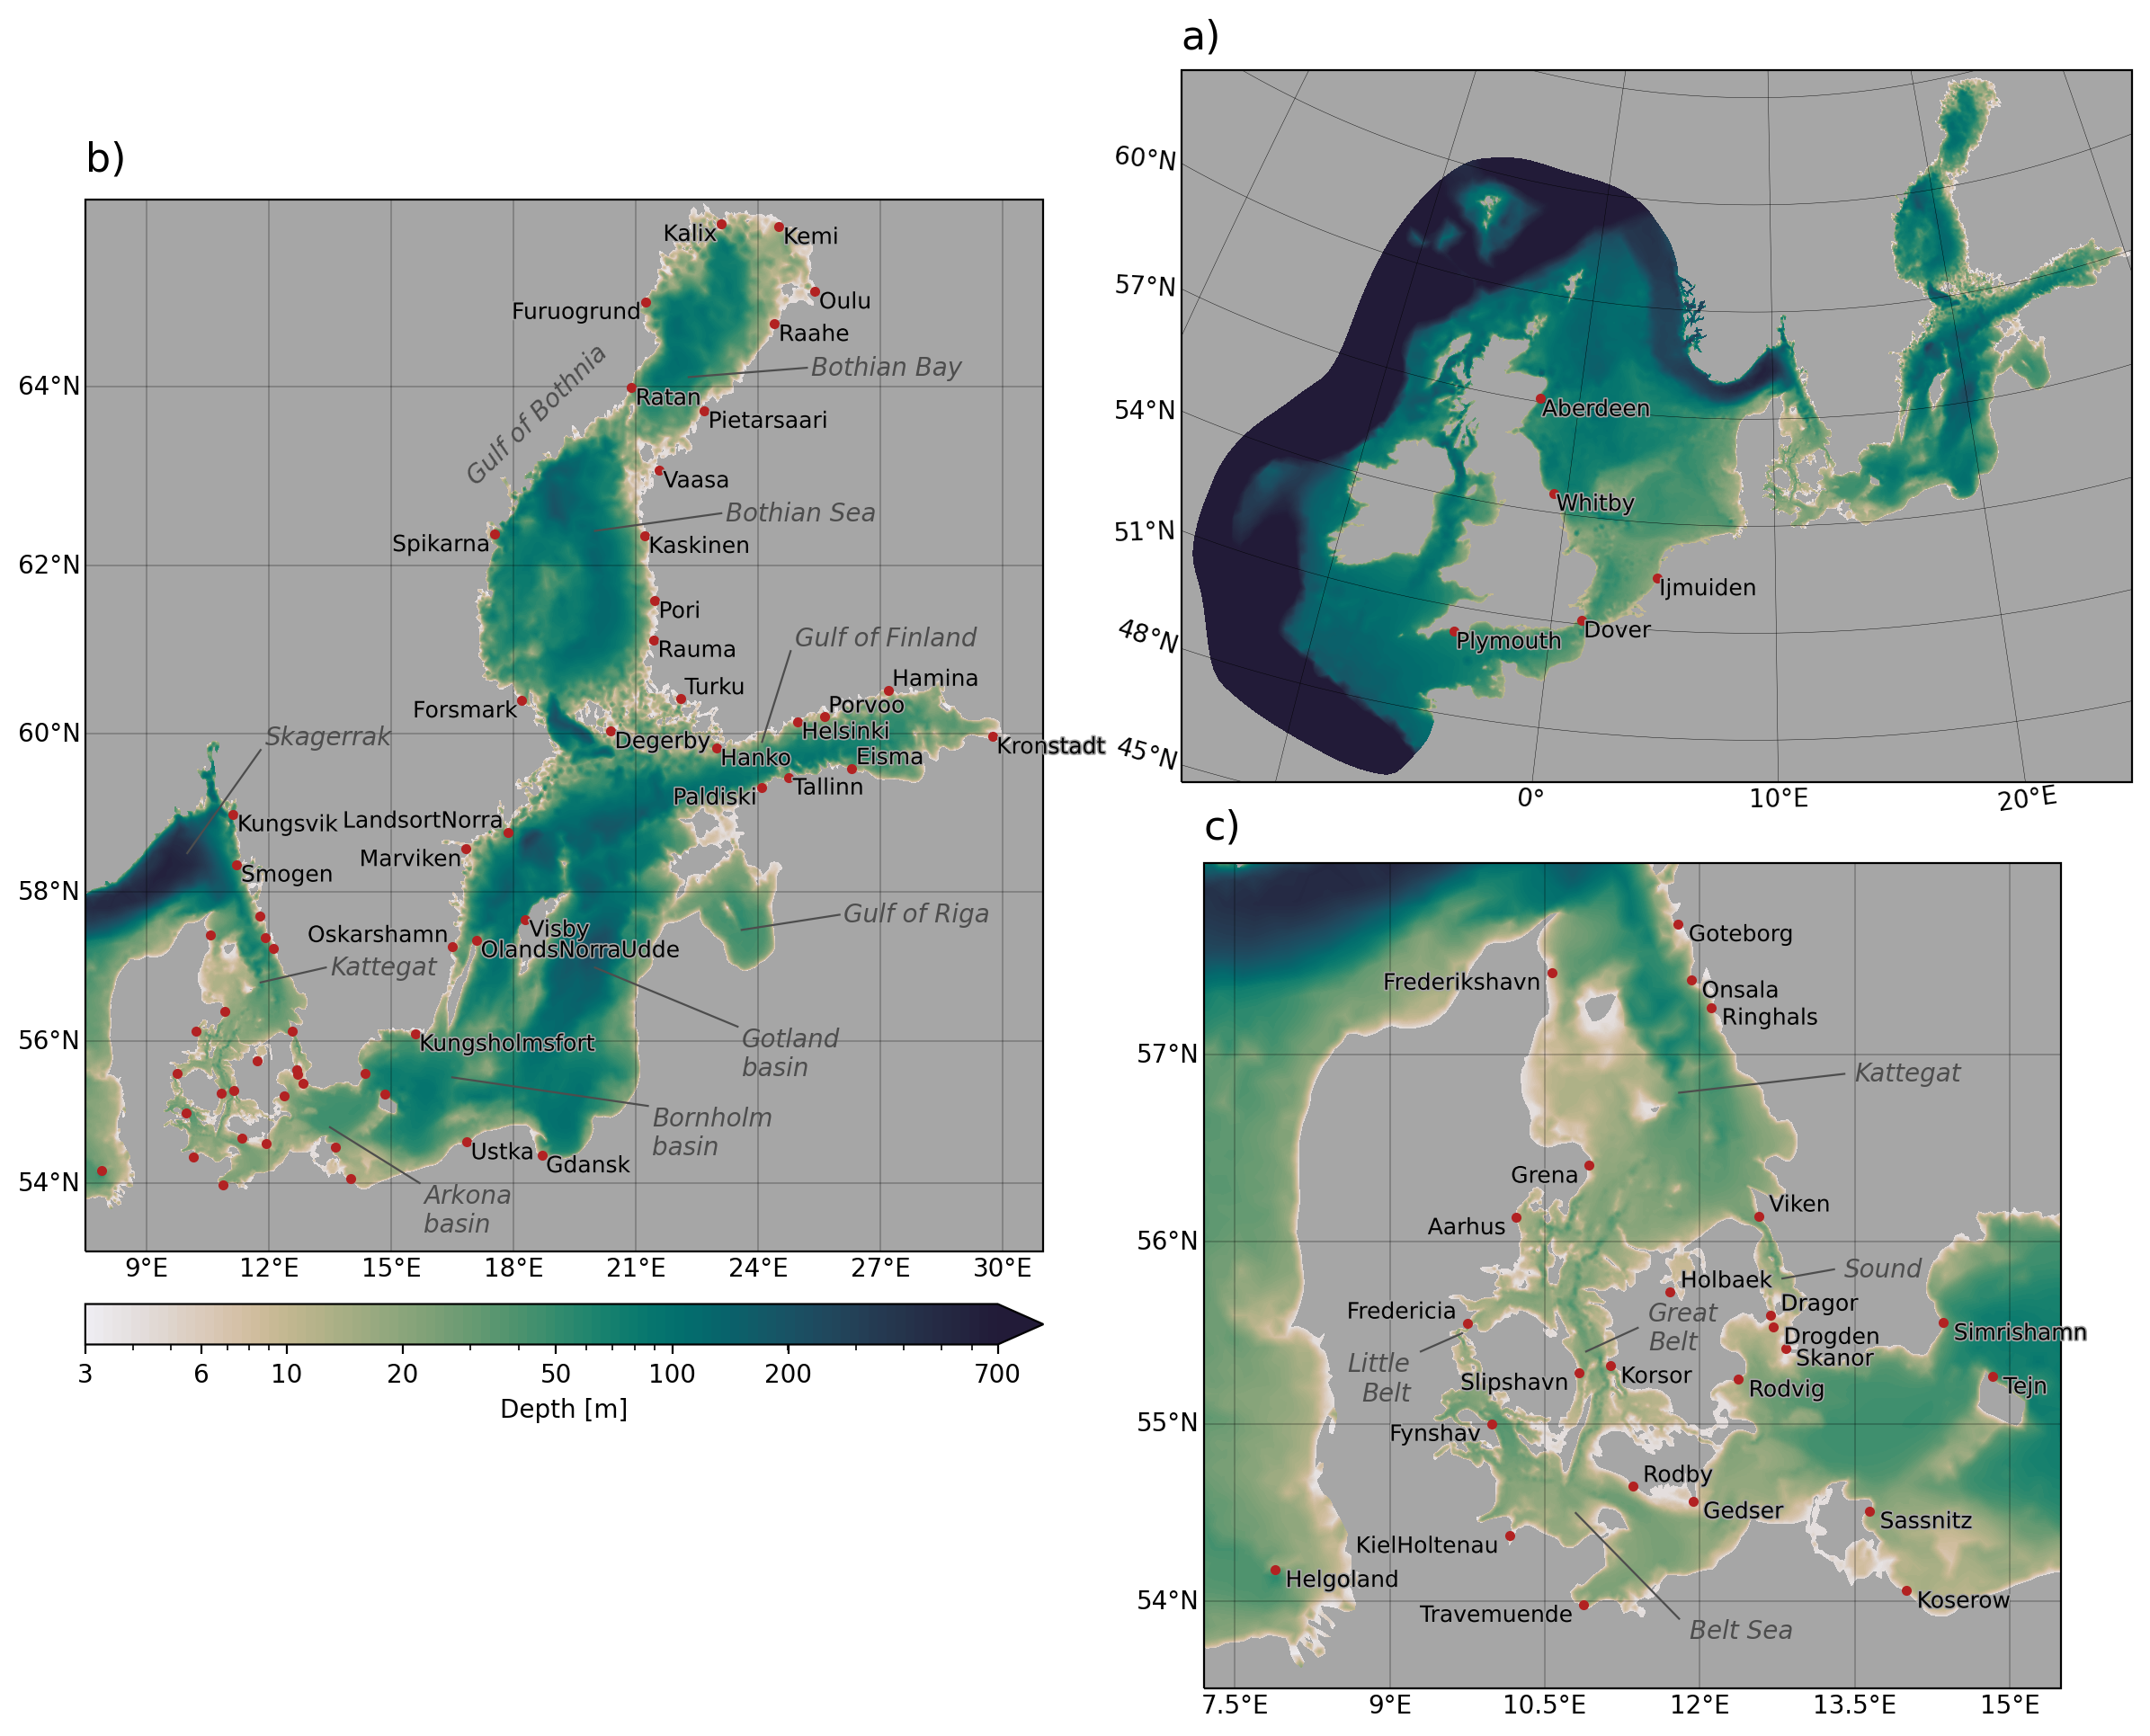
\includegraphics[width=1.1\textwidth]{domain}
\end{columns}
}

\frame{
\frametitle{Model configuration}
% \vspace*{-6mm}
\begin{columns}
 \column{0.48\textwidth}
 \begin{itemize}
  \item Unstructured mesh\\ resolution: 500 m .. 13 km
  \item Harmonie 2.5 km atmospheric forcing,\\ MSL pressure, 10 m winds
  \item Tides from global tidal model\\ (TPXO 9)
  \item River discharge (climatology),\\ 400+ rivers
  \item SSH comparison at 63 tide gauges
 \end{itemize}
 \column{0.53\textwidth}
  \hspace*{-5mm}
  \includegraphics[width=1.1\textwidth]{mesh_014_stations_baltic}
\end{columns}
}

\frame{
\frametitle{SSH Animation}
 \vspace*{-4mm}
 \begin{center}
  % \includegraphics[width=\textwidth]{}
 \movie[autostart,loop,open]
   {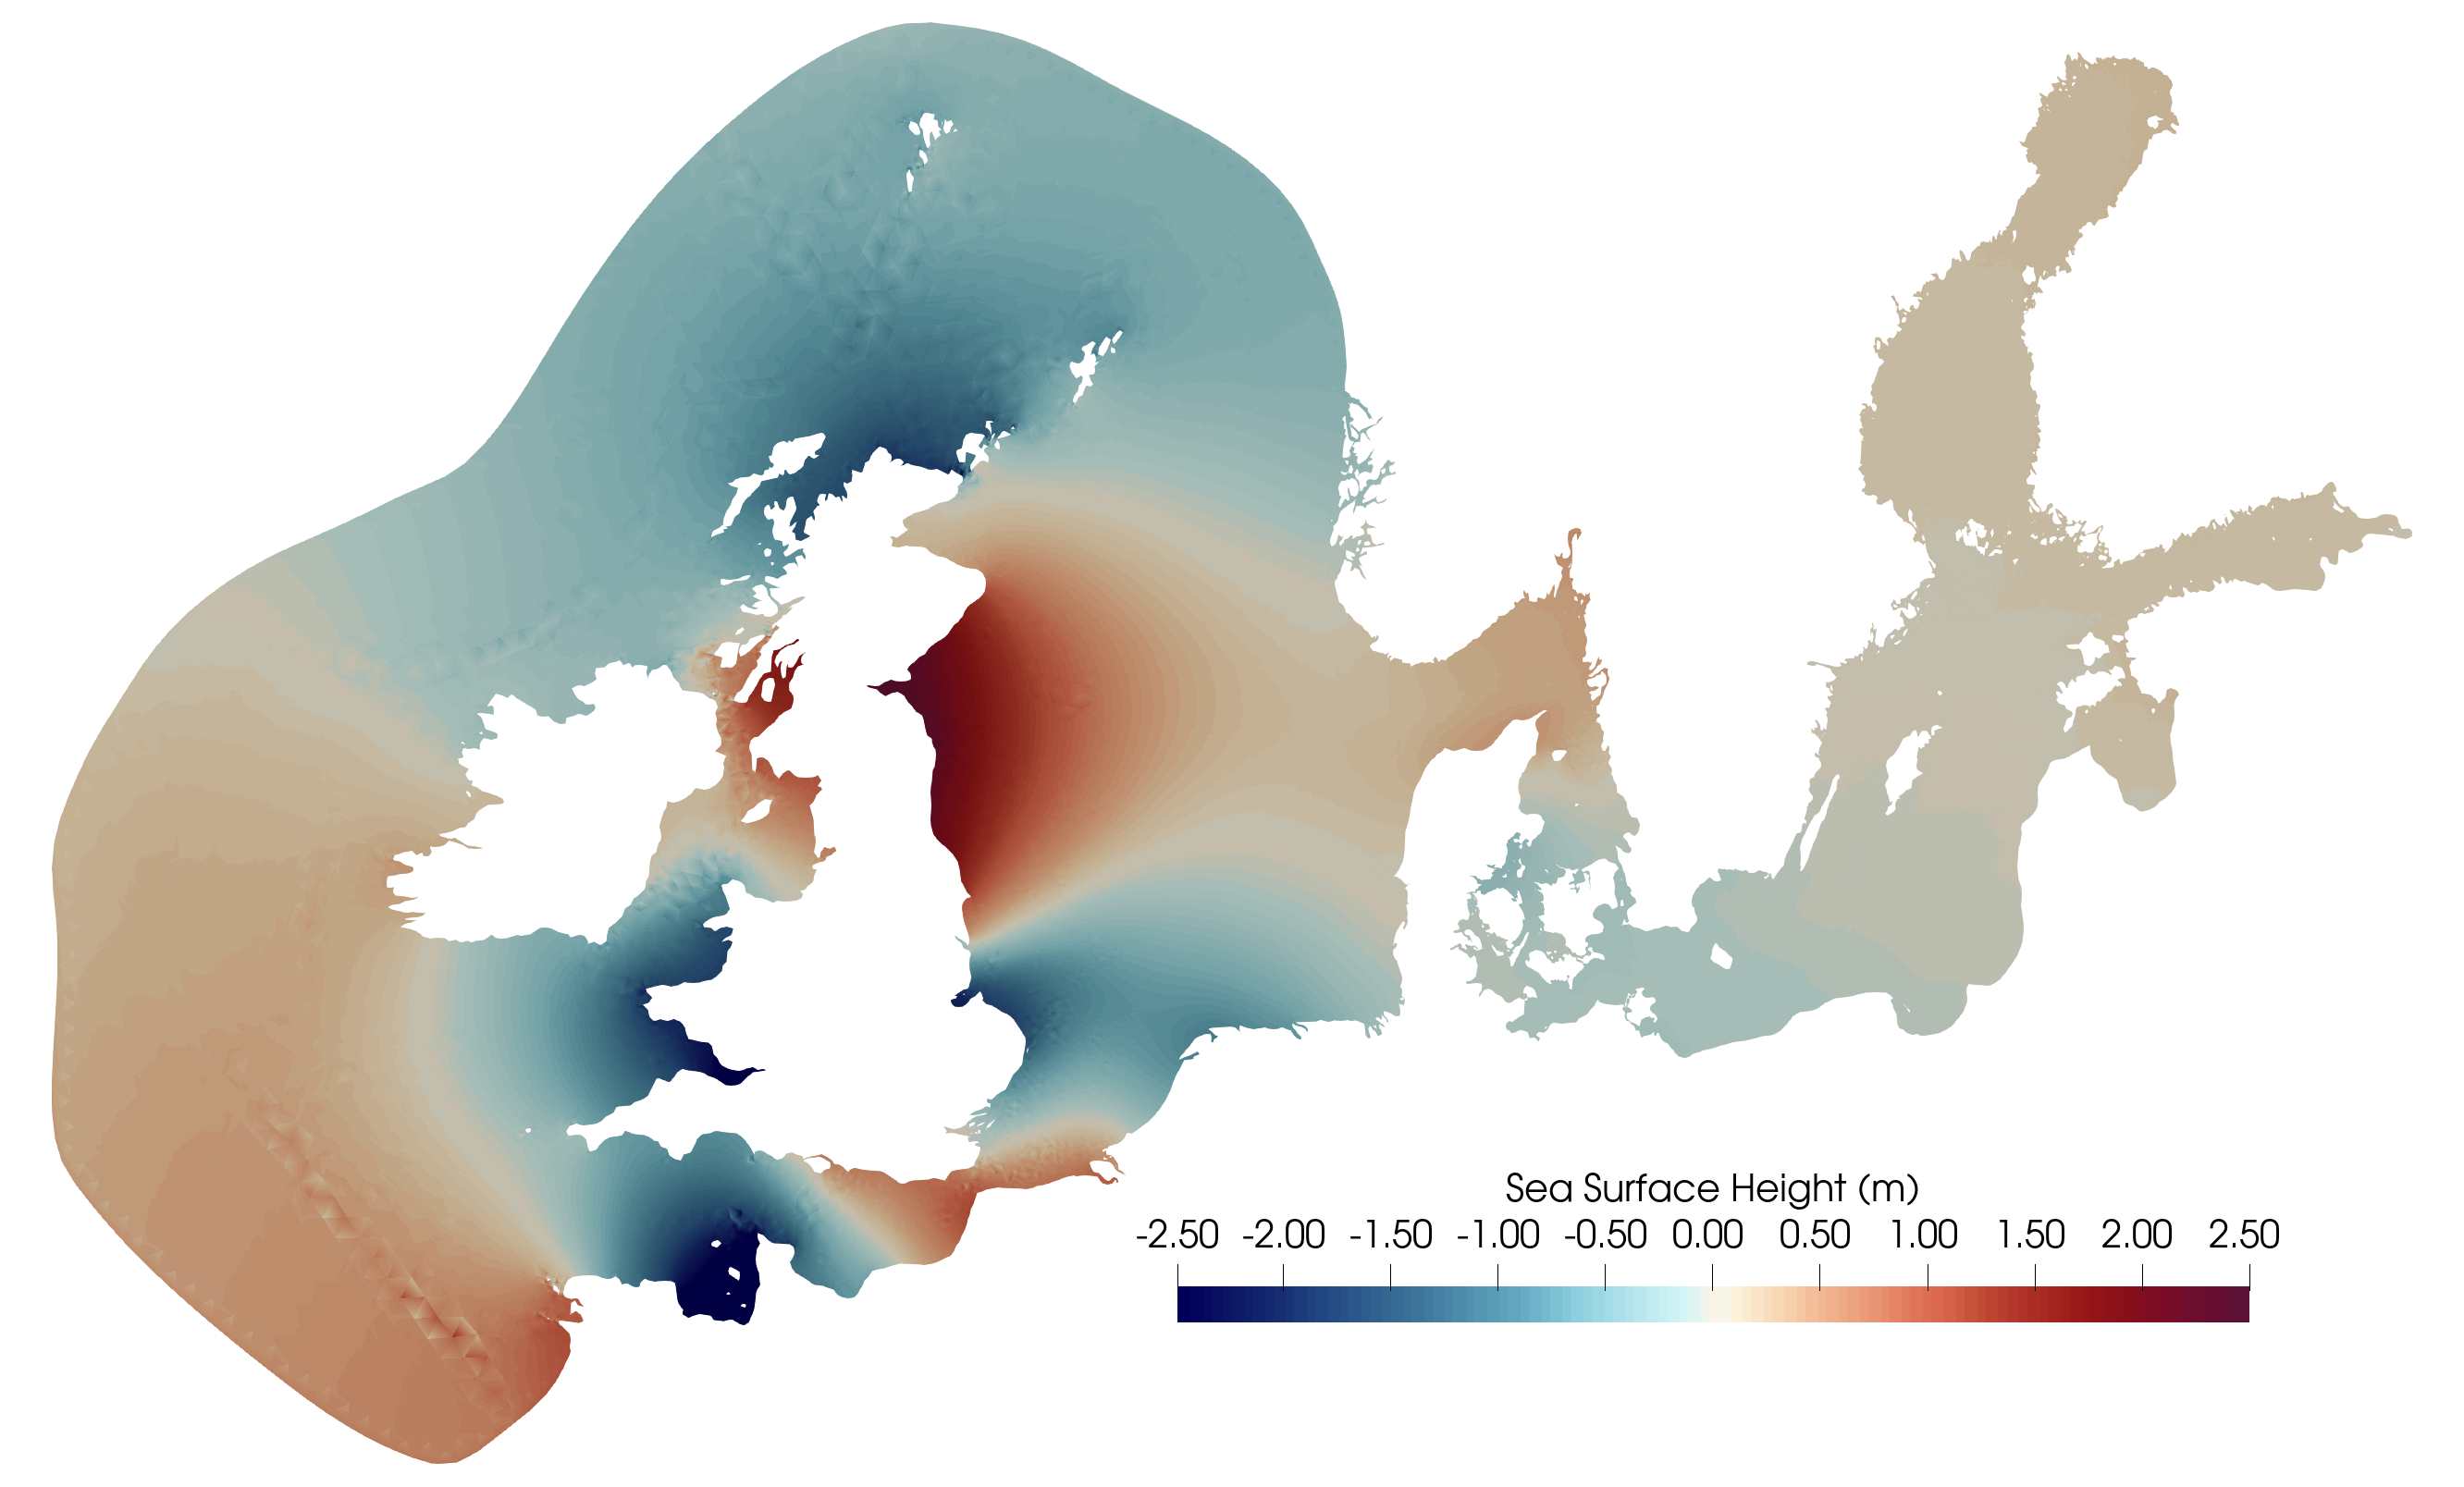
\includegraphics[width=0.95\textwidth]{animation_elev_m014_01_screenshot}}
   {animation_elev_m014_01.mp4}
  % \includemedia[
  %       width=13cm,height=7.2cm, %
  %       activate=pageopen,
  %       keepaspectratio,          % optionally useful
  %       playbutton=plain,
  %       addresource=animation_elev_m014_01.mp4,
  %       flashvars={
  %           source=animation_elev_m014_01.mp4
  %           &autoPlay=true
  %           &loop=true}
  %   ]{}{VPlayer.swf}
 \end{center}
}

\frame{
\frametitle{Optimizing bottom friction}
 \vspace*{-6mm}
 \begin{itemize}
  \item Cost function:
\begin{equation*}
 J(\mu) = \frac{1}{N_j N_i} \sum_{i,j} \frac{1}{Var(o_j)}((m_{j,i} - \overline{m_j}) - (o_{j,i} - \overline{o_j})^2 + J_{reg}
\end{equation*}
  \item Mean-Square-Deviation, Bias removed, Scaled by observation variance
  \begin{itemize}
   \item $o_{j,i}$, $m_{j,i}$: observation/model time series, $j$ stations, $i$ time steps
   \item $\overline{m_j})$ time average
  \end{itemize}
  \item $J_{reg}$ additional regularization term
  \item Control variable: Manning friction coefficient $\mu$
  \item Adjoint model provides the gradient $d J /d \mu$\\
        $\Rightarrow$ can use any gradient-based optimization method
 \end{itemize}
}

\frame{
\frametitle{Regularization}
 \vspace*{-6mm}
 \begin{itemize}
  \item Regularization term:
\begin{equation*}
 J_{reg}(\mu) = \alpha \|\mathbf{H}(\mu)\|_{2,1}^2 h^4 / A
\end{equation*}
  \item Squared norm of the Hessian matrix (2nd derivatives)
  \item $h$ is the local mesh element size, $A$ is total the mesh area
  \item Scaling $\alpha=400$ chosen to achieve a smoothly varying Manning coefficinet ($\mu$) field
 \end{itemize}
 \vspace*{5mm}
\emph{Best way to avoid over-fitting is to use a sufficiently long optimization period}
}

\frame{
\frametitle{Optimization results}
\small
\begin{columns}
 \column{0.5\textwidth}
Friction optimized with a Quasi-Newton iteration (L-BGFS)
\begin{itemize}
 \item Period: June 1 -- June 17, 2019
 \item Initial Manning coeff. = 0.03
 \item 40 iterations
\end{itemize}
Optimized Manning field
\begin{itemize}
 \item Large variability in the North-Sea; \\ $\rightsquigarrow$ Propagation of tides
 \item Lower friction in the Danish Straits; \\ $\rightsquigarrow$ Volume flux to Baltic Sea
 \item Higher friction in the Archipelago Sea; \\ $\rightsquigarrow$ Unresolved archpelago
\end{itemize}
 \column{0.5\textwidth}
 \hspace*{-4mm}
 \begin{overlayarea}{\textwidth}{0.9\textheight}
 \includegraphics<1>[width=1.0\textwidth]{progress_J_func}
 \includegraphics<2>[width=1.1\textwidth]{manning_field_full_i40}
 \includegraphics<3>[width=0.9\textwidth]{manning_field_ds_i40}
 \end{overlayarea}
\end{columns}
}

\frame{
\frametitle{Validation}
\framesubtitle{Optimization improves skill significantly}
\vspace*{-10mm}
\begin{columns}
 \column{0.4\textwidth}
    3 month simulation: \\
    June – August, 2019.
    \begin{itemize}
     \item Centralized Root Mean Square Deviation (CRMSD)
     \item Baltic Sea
     \begin{itemize}
      \item $< 6\ \text{cm}$
      \item typ. $\sim3\ \text{cm}$
     \end{itemize}
     \item Danish Straits (DS + Kat, $\star$)
     \begin{itemize}
      \item $< 8\ \text{cm}$
     \end{itemize}
     \item Standard deviation (STDDEV) close to observation {\footnotesize (black markers)}
    \end{itemize}
    \vspace{2mm}
    \emph{Overall performance comparable to best forecast models}
 \column{0.6\textwidth}
%  \vspace*{9.7mm}
 \begin{overlayarea}{\textwidth}{1.0\textheight}
 \includegraphics<1>[width=0.925\textwidth]{stats_slev_bswl-m014-01-bswl-m014-28-i40_2019-06-03_2019-08-31}
 \includegraphics<2>[width=\textwidth]{taylor_slev_bswl-m014-01-bswl-m014-28-i40_2019-06-03_2019-08-31}
 \end{overlayarea}
\end{columns}
}

\frame{
\frametitle{Validation: time series examples}
\small
\vspace*{-5mm}
\hspace*{-7mm}
 \alt<2>{
 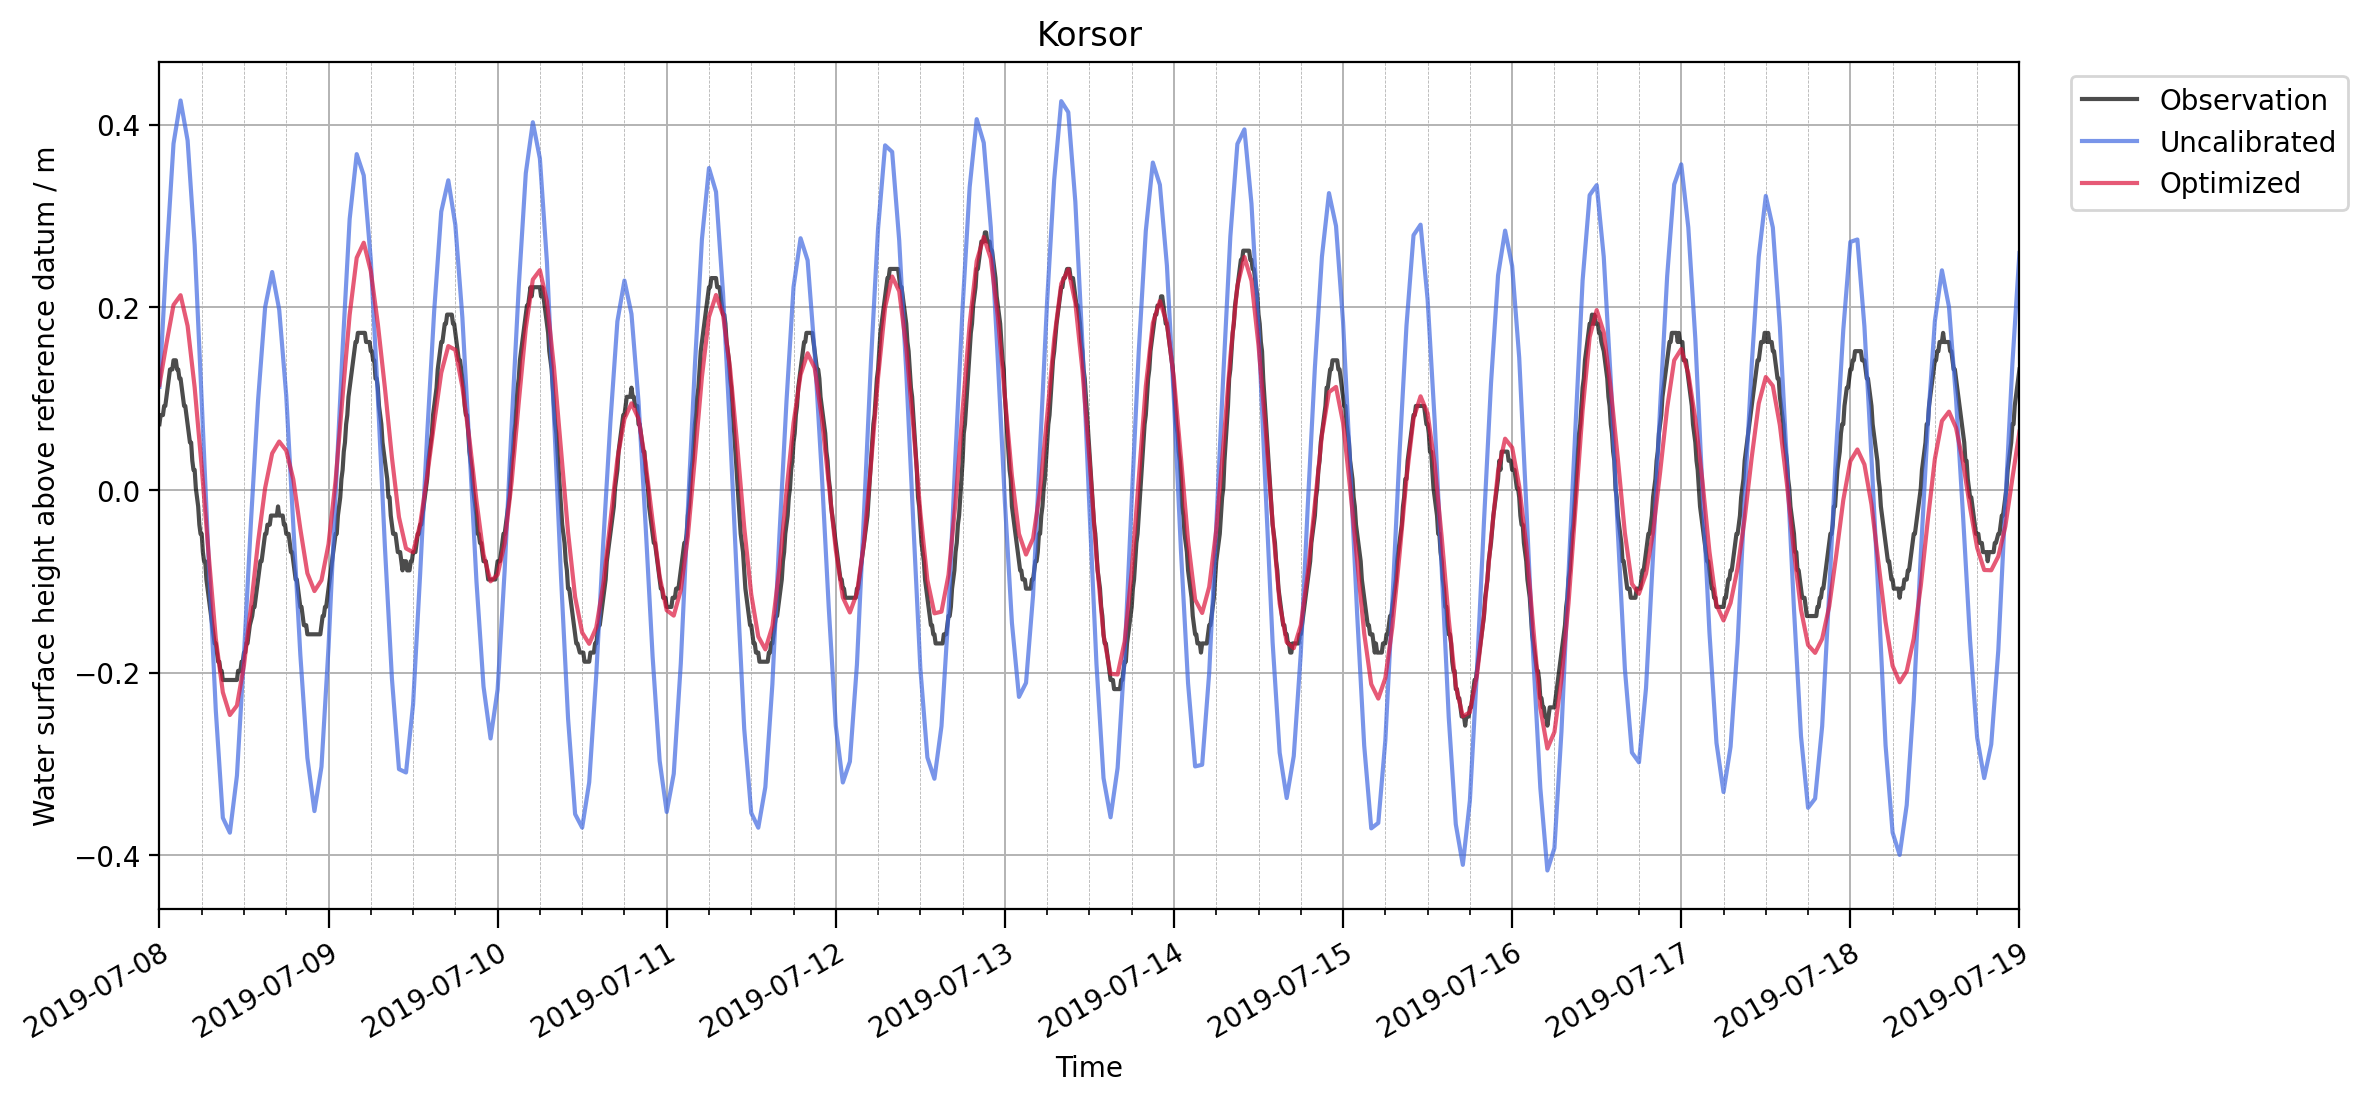
\includegraphics[width=1.1\textwidth]{ts_Korsor_d0m_slev_2019-07-08_2019-07-19}\\
 Correct tidal amplitude in the Danish Straits.
 }{
 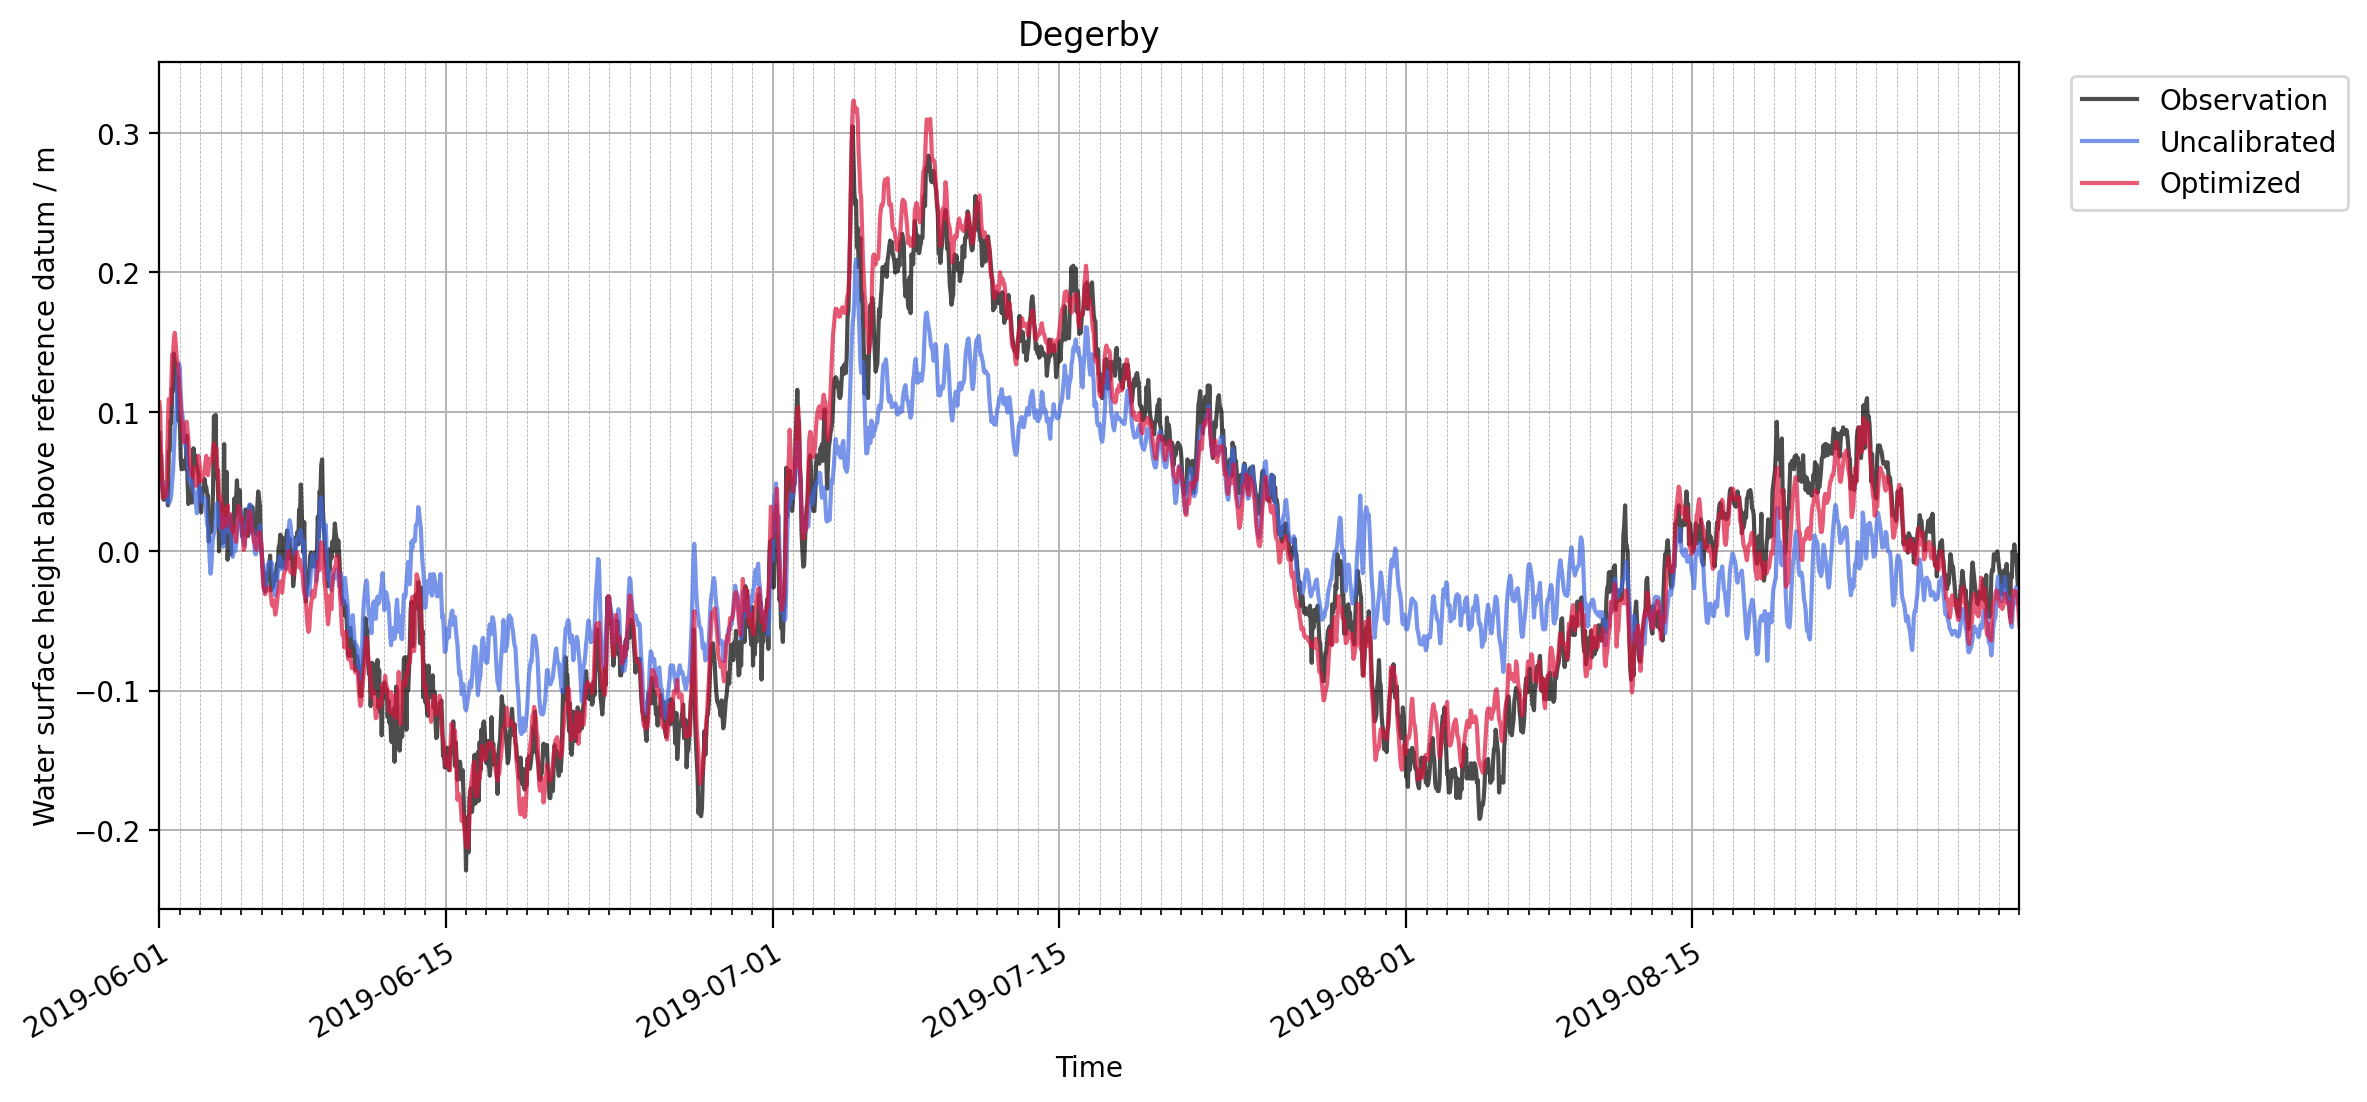
\includegraphics[width=1.1\textwidth]{ts_Degerby_d0m_slev_2019-06-01_2019-08-31}\\
 Correct wind-driven volume changes in the Baltic Sea.
 }
}

\frame{
\frametitle{Key take-home messages}
\emph{Adjoint-based parameter optimization works}\\[3mm]
Model configuration must be sufficiently good
 \begin{itemize}
  \item Mesh, bathymetry, forcings, initial condition\\
        $\Rightarrow$ error is dominated by the control variable (Manning coeff.)
 \end{itemize}
\visible<2->{
Cost function must be chosen carefully
 \begin{itemize}
  \item Measures the physical process of interest
  \item All stations should have equal weight
  \item Data preprocessing (whitening: bias removal and scaling)
 \end{itemize}
}
\visible<3->{
Regularization
 \begin{itemize}
  \item Sufficiently long optimization period (17 days)
  \item Additional penalization of 2nd derivatives (Hessian)
 \end{itemize}
}
}

\frame{
\frametitle{Conclusions}
2D water elevation model with an automatically-generated adjoint model
\begin{itemize}
 \item Results are encouraging
 \item Adjoint model is accurate and efficient
 \item Optimized bottom friction: excellent performance
\end{itemize}
Future work
\begin{itemize}
 \item Estimate initial condition (data assimilation)
 \item Error quantification
 \item Better optimization methods
 \item Extension to Thetis 3D model
\end{itemize}
\vspace*{6mm}
\emph{If you have any questions do not hesitate to contact me!\\
{\footnotesize\href{mailto:tuomas.karna@fmi.fi}{tuomas.karna@fmi.fi}}}
}

% \frame{
% \frametitle{Nemo-Nordic 2.0 operational marine model}
% % \vspace*{-6mm}
% \begin{columns}
%  \column{0.48\textwidth}
%  \begin{itemize}
%   \item Covers the North Sea and Baltic Sea
%   \item 1 nmi ($\sim$1.8 km) horizontal resolution
%   \item 56 vertical levels, $z^*$ partial cells
%   \item Surface resolution: 1 m
%   \item NEMO version 4.0
%  \end{itemize}
%  \column{0.53\textwidth}
%   \includegraphics[width=\textwidth]{domain_full}
% \end{columns}
% \vspace*{3mm}
% {\footnotesize
% Kärnä, T. et al., Nemo-Nordic 2.0: operational marine forecast model for the Baltic Sea, Geosci. Model Dev., 14, 5731–5749, \url{https://doi.org/10.5194/gmd-14-5731-2021}, 2021.
% }
% }

\end{document}
